\section{Model Evaluation and Selection}
\begin{multicols}{2}

\subsection{Evaluation metrics}
When we began working with supervised machine learning methods, we evaluated a classifier's performance using its accuracy. 

Accuracy, as you might recall, is the fraction of samples that were classified correctly. That is, where the classifier's predicted label matched the correct or true label. 

We also evaluated a regression model's performance using the default $R^2$ metric. 

In this module, you'll learn why measures like accuracy, which are simple and easy to understand, also have drawbacks. In that they don't give a complete enough picture of a supervised learning model's performance. And may not be the right metric for measuring success in your application. 

So we're going to cover several additional evaluation metrics beyond accuracy. We'll see how they're defined, what the motivation is for using them, and how to use them scikit-learn to get a better picture of how well a supervised model is doing on a given data set. You'll also learn how about to choose the right evaluation matrix for your application that can help you select the best model or find the optimal parameters. 

So let's return for a moment to this workflow diagram that we introduced earlier in the course. 

\begin{center}
    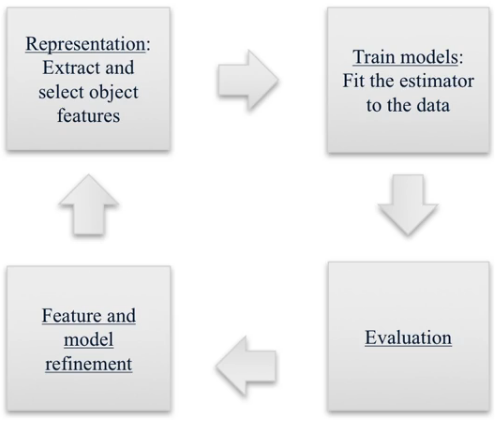
\includegraphics[width=\linewidth]{img/ML-cycle.png} 
\end{center}

You see that evaluation is a key part of this development cycle in applied machine learning. 

Once a model is trained, the evaluation step provides critical feedback on the trained model's performance characteristics. Particularly those that might be important for your application. 

The results of the evaluation step, for example, might help you understand which data instances are being classified or predicted incorrectly. Which might in turn suggest better features or different kernel function or other refinements to your learning model in the feature and model refinement phase. 

As we discussed earlier, the objective function that's optimized during the training phase may be a different, what's called \emph{a surrogate metric}. That's easier to use in practice for optimization purposes than what's used for the \emph{evaluation metric}. 

For example, a commercial search engine might use a ranking algorithm that is trained to recommend relevant web pages that best match a query. In other words, trying to predict a relevant label for a page. And that might be the objective in the \emph{training} phase. 

But there are many evaluation methods in the \emph{evaluation} phase that could be applied to measure aspects of that search engine's performance using that ranking algorithm, that are important to the search company's business, for example. Such as how many unique users the system sees per day. Or how long the typical user search session is and so on. 

So the \emph{evaluation measures} are the ones that in the end are used to select between different trained models or settings. 

Actually commercial search applications typically use a scorecard of multiple evaluation metrics to make important business decisions. Or development decisions about what models are chosen for use. 

So it's very important to choose evaluation methods that \emph{match} the goal of your application. 

For predicting the correct digit from a handwritten image, let's say, where each digit is equally likely, then accuracy may be a sufficient metric. 

However, there are other possible aspects of evaluation of model performance that are beyond average accuracy that may be critical to measure. For example, in a health application that uses a classifier to detect tumors in a medical image, we may want the classifier to error on the side of caution. And flag anything that even has a small chance of being cancerous. Even if it means sometimes incorrectly classifying healthy tissue as diseased. 

In this case, the classifier evaluation method would try to reduce what are called false negative predictions. 

We'll look at this in more detail shortly. 

More generally, your application goal might be based on very different metrics, such as user satisfaction, amount of revenue to your page, or increase in patient survival rates. 

So in the end, you'll be selecting the model or parameter settings that optimize those end evaluation metrics that are important to your goal. 

So in this module, we'll be focusing first on the widely used case of evaluating binary classification. And then we'll look at evaluation for the more general case of multi-class evaluation as well as regression. 

Before we start defining and using some evaluation metrics for binary classification, lets start by looking at example of why just looking at accuracy may not be enough to gain a good picture of what a classifier's doing. 

It'll also show us how knowing more about the types of errors a learning algorithm makes can help us get a better picture of a model's predictive performance. 

\subsection{Evaluation metrics for an imbalanced class}

First, let's consider the case where we have a binary classification task, where there are a lot of instances labeled with the negative class. But only a few instances that belong to the positive class. 

For example, we might see this scenario in online search or recommender systems. Where the system has to predict whether or not to display an advertisement or product suggestion. 

Or show a query suggestion or item on a page that's likely to be relevant given a user's query and what they clicked on in the past and so on. So those would be the positive examples. But of course there are many, many irrelevant items that are in the negative class that don't make sense to show a user. And so this is called an imbalanced class scenario. 

Another example might be datasets of credit card transactions. Where the vast majority of transactions are classified as normal and not fraud 

with a small minority of transactions that could be classified as fraudulent. 

These situations, which also apply to multi-class classification problems, involve datasets that have imbalanced classes. Imbalanced classes are very common in machine learning scenarios, so it's important to understand how to work with them. 

In particular, let's assume that we have an e-commerce application. Where for every 1,000 randomly sampled product items, one of them is relevant to a user's need and the other 999 are not relevant. 

So recall that accuracy computed over a set of instances is just the number of instances where the classifier's label prediction was correct divided by the total number of instances. 

Let's suppose you develop a classifier for predicting relevant e-commerce items. And after you've finished the development, you measure its accuracy on the test set to be 99.9\%. At first, that might seem to be amazingly good, right? That's incredibly close to perfect. 

But let's compare that to a dummy classifier that always just predicts the most likely class, namely, the not relevant class. In other words, no matter what the actual instance is, the dummy classifier will always predict that an item is not relevant. 

So if we have a test set that has 1,000 items, on average 999 of them will be not relevant anyway. So our dummy classifier will correctly predict the not relevant label for all of those 999 items. And so the accuracy of the dummy classifier is also going to be 99.9\%. So in reality our own classifier's performance isn't impressive at all. It's no better than just always predicting The majority class without even looking at the data. Let's take a look at another example of classification with imbalanced classes on a real dataset using our notebook. 

I'll start here using the digits dataset, which has images of handwritten digits labeled with ten classes, representing the digits zero through nine. 

As we can see by letting the dataset and then computing the count of instances in each class, using numpy's bin count method. There are roughly the same number of instances in each class. So this dataset has balanced classes. 

However with this digits dataset, now what we're going to do is create a new dataset with two imbalanced classes. By labelling all digits that are not the digit 1 as the negative class with label 0, and digits that are 1 as the positive class, label 1. So what I've done here is dump the first few entries from the original labels along with the new binary label, so you can see the imbalance visually. 

Now when we use bincount, we can see that there are about 1,600 negative examples, but only 182 positive examples. So indeed, we have a dataset that is class imbalanced. Or as expected almost exactly a nine to one ratio of negative to positive examples. 

Now let's create a train test partition on this imbalance set. And then train a support vector machine classifier with these binary labels using the radial basis function as a kernel. We get the accuracy using the score method, and we can see this is just over 90\%. Again at first glance, 90\% accuracy for a classifier seems pretty good. 

\subsection{A null accuracy baseline}

\subsubsection{With Dummy Classifier}

However, now let's create a Dummy Classifier that correctly reflect the class imbalance to see if 90\% really is that impressive. \texttt{scikit-learn} makes it easy to create a dummy classifier just by using the DummyClassifier class as shown here. 


{\scriptsize
\begin{verbatim}
from sklearn.dummy import DummyClassifier

# Negative class (0) is most frequent
dummy_majority=DummyClassifier(strategy='most_frequent')
dummy_majority.fit(X_train, y_train)
# Therefore the dummy 'most_frequent' classifier always 
# predicts class 0
y_dummy_predictions = dummy_majority.predict(X_test)
dummy_majority.score(X_test, y_test)
0.9044444444444445
\end{verbatim}
}

Dummy classifiers, again, are called that because they don't even look at the data to make a prediction. They simply use the strategy or rule of thumb that you instruct them to use, when creating them. In fact, when you create the classifier, you set the strategy argument to tell it what rule of thumb to use to make its predictions. So here, we set this to the most frequent strategy to predict the most frequent class. 

The DummyClassifier here is used just like a regular classifier. So to prepare it for prediction, we call the fit method on the \texttt{x_train} and \texttt{y_train} variables that hold the training set instances and labels. 

Now this DummyClassifier won't actually be looking at the individual data instances of those variables. But it does use the \texttt{y_train} variable to determine which class in the training data is most frequent. 

Finally, just like a regular classifier, we can call the predict method to make predictions on the test set. 

This example shows the output of the DummyClassifier's predictions. And as promised, you can see it's always predicting 0 or the negative class for every instance in the test set. 

Now we can call the usual score method to get the accuracy of the DummyClassifier's constant negative prediction. 

And we can see it's also 90\%, the same as our earlier support vector machine classifier with radio bases function kernel. 

So that support vector classifier was actually performing only very slightly better than the DummyClassifier. 

The dummy classifier provides what is called a null accuracy baseline. That is the accuracy that can be achieved by always picking the most frequent class. 

You should \emph{not} use a dummy classifier for real classification problems, but it does provide a useful sanity check in point of comparison. 

\subsubsection{Other Types of Dummy Classifiers}

There are other types of dummy classifiers that provide null base lines corresponding to other choices of the strategy parameter as shown here. 

\subsubsection*{Most frequent strategy}

Most frequent is the strategy we've just seen that always predicts the most frequent label. The stratified strategy, unlike the constant most frequent prediction is a random prediction that's based on the class distributions. For example, if the positive class occurs 90\% of the time in the training set. Then the stratified DummyClassifier will output the positive class label with 90\% probability. Otherwise, it will output the negative class label. 
This can help ensure that metrics that rely on having counts of both positive and negative class prediction outcomes can be computed. 

\subsubsection*{Uniform strategy}

The uniform strategy is another random prediction method that will generate class predictions uniformly at random. That is, all classes have an equal chance at being output as opposed to being weighed by their frequency in the training set. This strategy may be useful for gaining an accurate estimate of what the most common types of prediction errors for each class. 

\subsubsection*{Constant strategy}

The constant strategy can be useful when computing some metrics like F score, which we will cover in a few minutes. Well, why is that? Well, when we have a binary classification task where the most frequent class is the negative class. Turns out that using the most frequent strategy will never predict the positive class. And will never be able to count the number of positive instances that are correctly predicted. And so the overall count of such positive correct predictions will be 0. 

So this in turn as you will see in a few minutes, we'll cause some important metrics like \texttt{F scores} to always be zero. 

So using the constant strategy, we can force a dummy classifier to always predict the positive class even if it's the minority class in a set of classes. And this will lead to more meaningful computation of F-score. 

So what does it mean if we discover that our classifier has close to the DummyClassifier's performance? While typically it means that the features in our model may be ineffective, or erroneously computed or missing for some reason, it could also be caused by a poor choice of kernel or hyperparameter in the model. 

For example, if we change the support vector classifier's kernel parameter to \texttt{linear} from \texttt{rbf}. And recompute the accuracy on this retrain classifier, we can see that this leads to much better performance of almost 98\% compared to the most frequently class based line of 90\%. 

Finally, if you have accuracy that is close to that of a dummy classifier, it could be because there is indeed a large class \emph{imbalance}. And the accuracy gains produced by the classifier on the test set simply applied too few examples to produce a significant gain. 

In general, \textbf{for imbalanced} classification problems, you should use metrics \emph{other} than accuracy. We'll look at one shortly called AUC, which is short for area under the curve. 


\subsection{Binary Classification Outcomes}

Now let's look more carefully at the different types of outcomes we might see using a binary classifier. This will give us some insight into why using just accuracy doesn't give a complete picture of the classifier's performance. And will motivate our definition and exploration of additional evaluation metrics. 

With a positive and negative class, there are four possible outcomes that we can break into two cases corresponding to the first and second row of this matrix. 

If the true label for an instance is negative, the classifier can predict either negative, which is correct, and call the \textbf{true negative~--- TN}. Or it can erroneously predict positive, which is an error and called a \textbf{false positive~--- FP}. 

If the true label for an instance is positive, the classifier can predict either negative, which is an error and called a \textbf{false negative~--- FN}. Or it can predict positive, which is correct and that's called a \textbf{true positive~--- TP}. 

So maybe a quick way to remember this is that the first word in these matrix cells is false, if it's a a classifier error, or true if it's a classifier success. 

The second word is negative if the predicted label is negative and positive if the predicted label is positive. 

Another name for a false positive that you might know from statistics is a \textbf{type one error}. And another name for a false negative is a \textbf{type two error}. 

We'll also use capital \textbf{N} here to denote the total number of instances, of the sum of all the values in the matrix, the number of data points we're looking at. 

\begin{center}
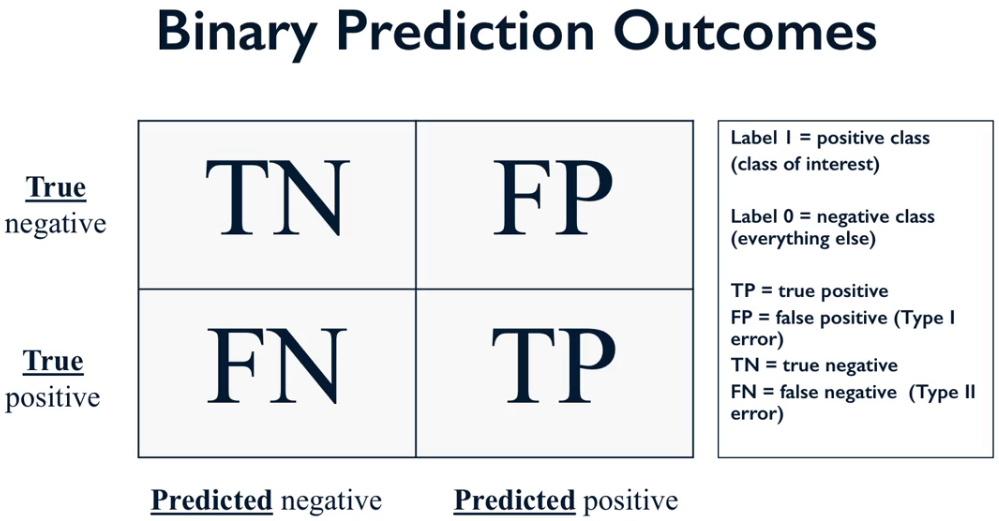
\includegraphics[width=\linewidth]{img/Binary-Prediction-Outcomes.png} 
\end{center}

This matrix of all combinations of predicted label and true label is called a \textbf{confusion matrix}. 

We can take any classifier prediction on a data instance and associate it with one of these matrix cells, depending on the true label of the instance and the classifier's predicted label. 

This also applies to multi-class classification, in addition to the special case of binary classification I've shown here. In the multi-class case with k classes, we simply have a k by k matrix instead of a two by two matrix. Scikit-learn makes it easy to compute a confusion matrix for your classifier. Let's take a look at the notebook. Here, we import the confusion matrix class from sklearn.metrics. We're going to use the same training set from the digits data set with the binary imbalance labels that we created earlier. 

To get the confusion matrix, we simply pass the \texttt{y_test} set of predicted labels and the y predicted set of predicted labels and then print the output. The order of the cells of the little matrix output here is the same as the one I just showed on the slide. 

True negative and false negative are in the first column, and true positive and false positive are in the second column. 

In particular, the successful predictions of the classifier are on the diagonal where the true class matches the predicted class. The cells off the diagonal represent errors of different types. 

Here, we compute the confusion matrices for different choices of classifier in the problem so we can see how they shift slightly with different choices of model. 

And this gives us some insight into the nature of successes and failures observed for each type of classifier. 

So first, we'll apply the most frequent class DummyClassifier we saw earlier. What we can see here is that the right column, that represent cases where the classifier predicted the positive class, is all zero. Which makes sense for this dummy classifier because it's always predicting the negative class, the most frequent one. We see that 407 instances are true negatives, and there are 43 errors that are false negatives. 

Here we apply the stratified DummyClassifier that gives random output in proportion to the ratio labels in the training set. Now the right column is no longer all zero because this DummyClassifier does predict occasionally predict the positive class. If we add the numbers in the right column, we see that 32 plus 6 equals 38 times the number of times the classifier predicted the positive class. Of those times, in six cases, the lower right diagonal, this was a true positive. 

In the next case, we'll apply a support vector classifier with linear kernel and seed parameter equal to one. 

We note that looking along the diagonal compared to the stratified dummy classifier above, which had a total of 375 plus 6, or 381 correct predictions. The support vector classifier has a total of 402 plus 38, which is 440 correct predictions on the same data set. 

Likewise, we can apply a logistic regression classifier, and that obtains similar results to the support vector classifier. And finally, we can apply a decision tree classifier, and look at the confusion matrix that results from that. One thing we notice is, that unlike the support vector or logistic regression classifier, which had balanced numbers of false negatives and false positives. The decision tree makes more than twice as many false negative errors, 17 of them actually, as false positive errors, of which there are 7. Now that we've seen how a confusion matrix can give us a little more information about the types of errors a classifier makes, we're ready to move ahead and and define some new types of evaluation metrics that use information from the computing matrix to give different perspectives on classifier performance.

\end{multicols}